\documentclass[12pt]{article}
\usepackage[utf8]{inputenc}
\usepackage[spanish]{babel}
\usepackage{amsmath}
\usepackage{amsthm}
\usepackage{amssymb}
\usepackage{fancyhdr}
\usepackage{mathpazo,amsfonts}
\usepackage[margin=0.95in]{geometry}
\usepackage{tikz}


\usepackage[
backend=biber,
style=alphabetic,
sorting=ynt
]{biblatex}

\addbibresource{blb.bib}

\pagestyle{fancy}

\lhead{Tarea 1}
\chead{Nora Toussaint y Luis González}
\rhead{18 de febrero de 2022}

\newcommand{\N}{\mathbb{N}}
\newcommand{\Z}{\mathbb{Z}}
\newcommand{\Q}{\mathbb{Q}}
\newcommand{\R}{\mathbb{R}}

\newtheorem{prop}[section]{Proposición}

\newenvironment{problem}[2][Problema]{\begin{trivlist}
\item[\hskip \labelsep {\bfseries #1}\hskip \labelsep {\bfseries #2.}]}{\end{trivlist}}

\begin{document}
\section*{Teoría de Gráficas}

%---------------------------------
\begin{problem}{1.1.7} El \textit{n-cubo} $Q_n$ ($n\geq 1)$ es la gráfica cuyos vértices son el conjunto de $n-$tuplas de $0$s y $1$s, donde dos $n-$tuplas son adyacentes si estas difieren precisamente en una coordenda.
\begin{itemize}
    \item[a)] Dibuje $Q_1, Q_2, Q_3$ y $Q_4.$
    \item[b)] Determine $v(Q_n)$ y $e(Q_n).$
    \item[c)] Demuestre que $Q_n$ es bipartita para toda $n\geq 1.$
\end{itemize}
\end{problem}
\textit{Solución.}
\begin{itemize}
    \item[a)] Las representaciones de estas gráficas pueden verse en la Figura \ref{fig:fig4}.
    
    \begin{figure}[h]
        \centering
        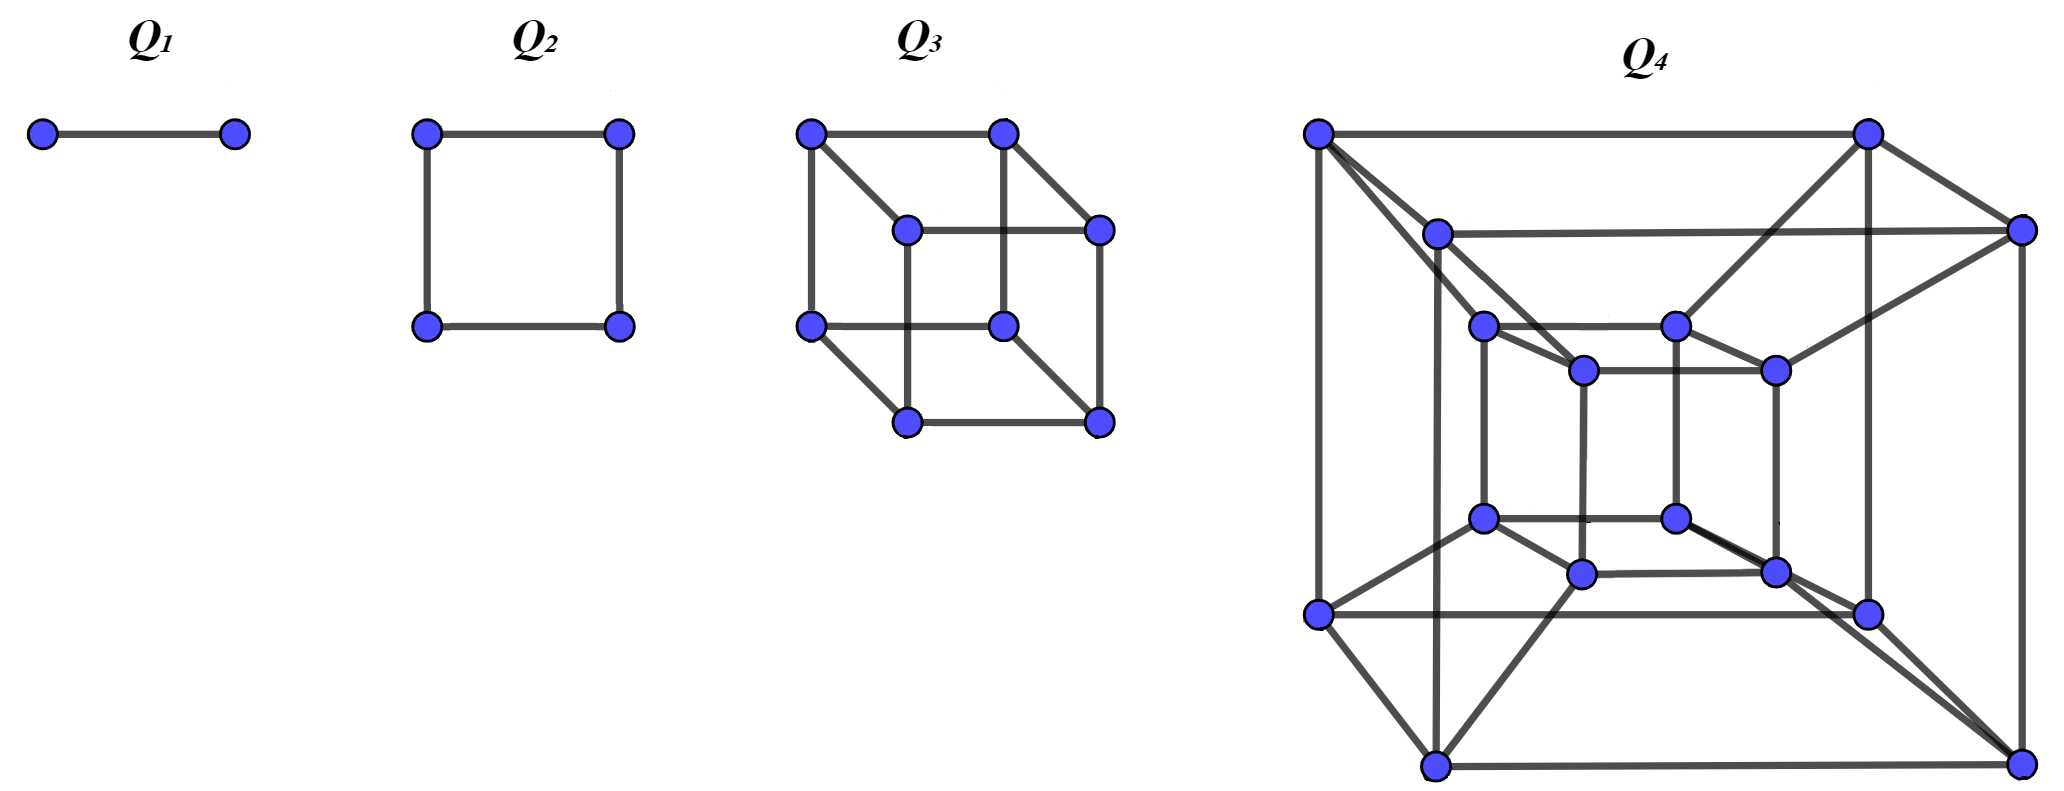
\includegraphics[scale=0.45]{pics/graph2.png}
        \caption{Gráficas $Q_1, Q_2, Q_3$ y $Q_4.$}
        \label{fig:fig4}
    \end{figure}
    \item[b)] Sea $v$ es un vértice de $Q_n$. Por definición, $v$ tiene $n$ coordenadas, cada una con dos valores posibles. Luego, el número de vértices distintos de $Q_n$ es $2^n.$
    
    Por otro lado, los vértices adyacentes a $v$ son aquellos que difieren exactamente en una coordenada respecto a $v$. Siendo $v$ una $n-$tupla, tenemos $n$ vértices adyacentes a $v.$ En general, $Q_n$ es $n$-regular. Luego,
    $$e(Q_n) = \frac{1}{2} \sum_{v \in V} d(v) = \frac{1}{2} \left(2^n \cdot n\right) = n 2^{n-1}.$$
    \item[c)] Sean $X = \{(v_1,\ldots, v_n): \sum_{i=1}^n v_i \text{ es par}\}$ y $Y = \{(v_1,\ldots, v_n): \sum_{i=1}^n v_i \text{ es impar}\}$. Estos conjuntos forman una partición del conjunto de vértices de $Q_n.$ De manera que si $(u_1,\ldots,u_n)(v_1,\ldots, v_n)$ es una arista de $Q_n$, sin pérdida de generalidad podemos asumir que $(u_1,\ldots,u_n)$ está en $X.$ Por definición de $Q_n$, el vértice $(v_1, \ldots, v_n)$ difiere en exactamente una coordenada con respecto al vértice $(u_1,\ldots, u_n).$ Luego, $ \sum_{i=1}^n u_i = 1 \pm \sum_{i=1}^n v_i$, según sea el caso. Por tanto, el extremo $(u_1,\ldots, u_n)$ pertenece a $Y$. Concluimos que $Q_n$ es bipartita.
\end{itemize}
%---------------------------------

%---------------------------------
\begin{problem}{1.1.9} Sea $G[X,Y]$ una gráfica bipartita.
\begin{itemize}
    \item[a)] Demuestre que $\sum_{v\in X} d(v) = \sum_{v\in Y} d(v).$
    \item[b)] Deduzca que si $G$ es $k-$regular, con $k\geq 1$, entonces $\lvert X \rvert = \lvert Y \rvert.$
\end{itemize}
\end{problem}
\begin{proof}
\text{ }
\begin{itemize}
    \item[a)] Sea $\boldsymbol{B}$ la matriz de adyacencia bipartita de $G[X,Y]$. Observe que la suma de los elementos de la fila correspondiente a $x\in X$ es igual a $d(x)$. De igual forma, la suma de los elementos de la columna correspondiente a $y\in Y$ es igual a $d(y).$ Así pues, la suma por filas es igual a $\sum_{v\in X} d(v)$; y esta debe ser igual a la suma de culumnas $\sum_{v \in Y} d(v)$.
    
    \item[b)] Como $G[X, Y]$ es $k-$regular, se tiene que $d(v) = k \geq 1$ para todo $v \in V$. Luego, por la Proposición 1.3 de \cite{10.5555/1481153} se tiene que $\lvert X \rvert = \lvert Y \rvert$.
\end{itemize}
\end{proof}
%---------------------------------

%---------------------------------
\begin{problem}{1.1.10} Sea $G$ una gráfica simple y $k-$partita con partes de tamaño $a_1, a_2, \ldots, a_k.$ Demuestre que $m\leq \frac{1}{2} \sum_{i=1}^k a_i(n-a_i).$
\end{problem}
\begin{proof}
Sea $G[X_1,\ldots, X_k]$ una gráfica $k-$partita con $\lvert X_i \rvert = a_i$ para $i=1,\ldots,k$. Tenemos que

\begin{eqnarray*}
m &=& \frac{1}{2} \sum_{v \in V(G)} d(v)\\
&=& \frac{1}{2} \sum_{i=1}^k \sum_{v \in V(X_i)} d(v)\\
&\leq& \frac{1}{2} \sum_{i=1}^k \sum_{v \in V(X_i)} (n - a_i)\\ 
&=& \frac{1}{2} \sum_{i=1}^k a_i(n-a_i),
\end{eqnarray*}
donde la desigualdad anterior se obtiene dado que para cualquier vértice $v$ en $X_i$ ($i=1, \ldots, k$) existen a lo más $(n-a_i)$ aristas incidentes posibles.
\end{proof}
%---------------------------------

%---------------------------------
\begin{problem}{1.1.11} \text{ }
\begin{itemize}
    \item[a)] Demuestre que $T_{k,n}$ tiene más aristas que cualquier otra gráfica simple completa $k-$partita.
    \item[b)] Determine $e(T_{k,n})$.
\end{itemize}
\end{problem}
\begin{proof} Para este problema, $T_{n,k}$ es una gráfica de Turán en $n$ vértices con $k$ partes.
\begin{itemize}
    \item[a)] Sea $G[X_1, \ldots, X_k]$ una gráfica simple $k-$partita completa con $\lvert X_i \rvert = a_i$ para $i\in \{1, \ldots, k\}$. Además, suponga que existen $i,j$ en $\{1,\ldots, k\}$ tales que $a_i - a_j  \geq 2$. Sea $v \in X_i$ y definamos $H[Y_1, \ldots, Y_k]$ como la gráfica simple $k-$partita completa con $Y_i = X_i - \{v\}$, $Y_j = X_j \cup \{v\}$ y $Y_r = X_r$ para $r\in\{1,\ldots, k\}$ diferente de $i$ y de $j.$ Entonces \footnote{Estamos usando, como corolario al Problema 1.1.10, que $e(G) = \frac{1}{2}\sum_{i=1}^k a_i (n-a_i).$}
    \begin{eqnarray*}
    e(H) - e(G) &=& \frac{1}{2}[(a_i-1)(n-a_i+1) + (a_j+1)(n - a_j - 1)] - [a_i(n-a_i) + a_j(n-a_j) ]\\
    &=& a_i-a_j-1 \\
    &\geq& 1.
    \end{eqnarray*}
    Por tanto, $e(H) > e(G).$ Más aún, lo anterior muestra que las gráficas simples $k-$partitas completas cuyas partes tienen tamaños que difieren a lo más por $1$ son máximas en aristas. Pero estas son precisamente las gráficas de Turán.
    
    \item[b)] Por el algoritmo de Euclides, existen enteros $q$ y $r$ tales que $n = kq + r$ con $0 \leq r < k$. Entonces, existen $r$ partes de tamaño $q+1$ y $k-r$ partes de tamaño $q.$ Luego,
    
    \begin{eqnarray*}
    e(T_{k,n}) &=& \frac{1}{2} \left[ r(q+1)(n-q-1) + (k-r) q(n-q) \right] \\
    &=& \frac{1}{2} \left[ n^2 - nq - r(q+1) \right] \\ 
    &=& \frac{1}{2} \left(n^2 - n \left\lfloor \frac{n}{k} \right\rfloor - r \left\lceil \frac{n}{k} \right\rceil \right).
    \end{eqnarray*}
\end{itemize}
\end{proof}
%---------------------------------

%---------------------------------
\begin{problem}{1.1.13} \text{ }
\begin{itemize}
    \item[a)] Demuestre que si $G$ es simple y $\delta > \frac{1}{2}(n-2),$ entonces $G$ es conexa. 
    \item[b)] Para $n$ par, encuentre una gráfica simple no conexa y $\frac{1}{2}(n-2)-$regular.
\end{itemize}
\end{problem}
\begin{proof}\text{ }
\begin{itemize}
    \item[a)] Sea $G$ gráfica simple con $\delta > \frac{1}{2}(n-2)$ y suponga que es no conexa. Entonces existe una partición  $X$ y $Y$ de los vértices de $G$ de tal manera que ningún vértice de $X$ es adyacente a ningún vértice de $Y$. Si $v$ es un vértice de $X$, entonces $d(v) > \frac{1}{2}(n-2)$. Luego, $\lvert X\rvert > \frac{1}{2}(n-2) + 1 = \frac{n}{2}.$ De manera similar, se tiene que $\lvert Y \rvert > \frac{n}{2}.$ Pero entonces $\lvert G \rvert  = \lvert X \rvert + \lvert Y \rvert > n$, lo cual es una contradicción. Por tanto, $G$ es conexa.
    \item[b)] Consideremos la gráfica $G$ con dos componentes conexas iguales a $K_{\frac{n}{2}}.$  Esta gráfica es $\frac{1}{2}(n-2)$-regular, simple y no conexa. 
\end{itemize}
\end{proof}
%---------------------------------

%---------------------------------
\begin{problem}{1.1.17}
Sea $G$ una gráfica simple. El complemento $\overline{G}$ de $G$, es la gráfica simple cuyos vértices son $V$ y cuyas aristas son todas las parejas de vértices no adyacentes. \begin{itemize}
    \item[a)] Encuentre la sucesión de grado de $\overline{G}$ en términos de la sucesión de grado de $G$.
    \item[b)] Demuestre que si $G$ es no conexa, entonces $\overline{G}$ es conexa. ¿El converso es cierto?
\end{itemize}
\end{problem}
\begin{proof} \text{ }
\begin{itemize}
    \item[a)] Sea $(d(v_1), \ldots, d(v_n))$ la sucesión de grados de $G$. Observe que para toda $i \in \{1, \ldots, n\}$, existen $n - d(v_i) - 1$ aristas incidentes a $v_i$ en $\overline{G}$. Por tanto, la sucesión de grados de $\overline{G}$ es $(n-d(v_1)-1, \ldots, n-d(v_n)-1).$

    \item[b)] Suponga que $G$ es simple y no conexa. Sea $\{X,Y\}$ una partición de $V(\overline{G})$. Como $V(\overline{G}) = V(G)$ y $G$ es no conexa, existen $x\in X$ y $y \in Y$ no adyacentes. Entonces $xy \in E(\overline{G})$. Como $X, Y$ es una partición arbitraria de $V(\overline{G})$, concluimos que $\overline{G}$ es conexa. 
    
    El converso es falso. Por ejemplo, la gráfica $\overline{C_5}$ es conexa y  $C_5$ también, tal y como se muestra en la Figura \ref{fig:fig2}. 
\end{itemize}
\end{proof}

\begin{figure}[h]
    \centering
\tikzset{every picture/.style={line width=0.75pt}} %set default line width to 0.75pt        

\begin{tikzpicture}[x=0.75pt,y=0.75pt,yscale=-1,xscale=1]
%uncomment if require: \path (0,300); %set diagram left start at 0, and has height of 300

%Shape: Regular Polygon [id:dp6861666567021985] 
\draw   (266.12,203.64) -- (176.19,203.14) -- (148.88,117.45) -- (221.93,65) -- (294.39,118.27) -- cycle ;
%Shape: Circle [id:dp9157590012435128] 
\draw  [fill={rgb, 255:red, 255; green, 255; blue, 255 }  ,fill opacity=1 ] (216.18,65) .. controls (216.18,62.25) and (218.41,60.01) .. (221.17,60.01) .. controls (223.92,60.01) and (226.16,62.25) .. (226.16,65) .. controls (226.16,67.76) and (223.92,69.99) .. (221.17,69.99) .. controls (218.41,69.99) and (216.18,67.76) .. (216.18,65) -- cycle ;
%Shape: Circle [id:dp809511444895484] 
\draw  [fill={rgb, 255:red, 255; green, 255; blue, 255 }  ,fill opacity=1 ] (289.4,118.27) .. controls (289.4,115.51) and (291.63,113.28) .. (294.39,113.28) .. controls (297.14,113.28) and (299.38,115.51) .. (299.38,118.27) .. controls (299.38,121.02) and (297.14,123.26) .. (294.39,123.26) .. controls (291.63,123.26) and (289.4,121.02) .. (289.4,118.27) -- cycle ;
%Shape: Circle [id:dp8556736803258348] 
\draw  [fill={rgb, 255:red, 255; green, 255; blue, 255 }  ,fill opacity=1 ] (261.13,203.64) .. controls (261.13,200.88) and (263.36,198.65) .. (266.12,198.65) .. controls (268.87,198.65) and (271.11,200.88) .. (271.11,203.64) .. controls (271.11,206.4) and (268.87,208.63) .. (266.12,208.63) .. controls (263.36,208.63) and (261.13,206.4) .. (261.13,203.64) -- cycle ;
%Shape: Circle [id:dp9686444751658032] 
\draw  [fill={rgb, 255:red, 255; green, 255; blue, 255 }  ,fill opacity=1 ] (143.89,117.45) .. controls (143.89,114.7) and (146.12,112.47) .. (148.88,112.47) .. controls (151.63,112.47) and (153.87,114.7) .. (153.87,117.45) .. controls (153.87,120.21) and (151.63,122.44) .. (148.88,122.44) .. controls (146.12,122.44) and (143.89,120.21) .. (143.89,117.45) -- cycle ;
%Shape: Circle [id:dp9167700799683631] 
\draw  [fill={rgb, 255:red, 255; green, 255; blue, 255 }  ,fill opacity=1 ] (171.2,203.14) .. controls (171.2,200.38) and (173.43,198.15) .. (176.19,198.15) .. controls (178.94,198.15) and (181.18,200.38) .. (181.18,203.14) .. controls (181.18,205.89) and (178.94,208.13) .. (176.19,208.13) .. controls (173.43,208.13) and (171.2,205.89) .. (171.2,203.14) -- cycle ;
%Straight Lines [id:da18237736326068776] 
\draw    (428.17,66) -- (473.12,204.64) ;
%Straight Lines [id:da7699040218562152] 
\draw    (355.88,118.45) -- (501.39,119.27) ;
%Straight Lines [id:da988317687849227] 
\draw    (383.19,204.14) -- (501.39,119.27) ;
%Straight Lines [id:da7825041577968535] 
\draw    (383.19,204.14) -- (428.17,66) ;
%Straight Lines [id:da874256935943281] 
\draw    (473.12,204.64) -- (355.88,118.45) ;
%Shape: Circle [id:dp09940496208575422] 
\draw  [fill={rgb, 255:red, 255; green, 255; blue, 255 }  ,fill opacity=1 ] (350.89,118.45) .. controls (350.89,115.7) and (353.12,113.47) .. (355.88,113.47) .. controls (358.63,113.47) and (360.87,115.7) .. (360.87,118.45) .. controls (360.87,121.21) and (358.63,123.44) .. (355.88,123.44) .. controls (353.12,123.44) and (350.89,121.21) .. (350.89,118.45) -- cycle ;
%Shape: Circle [id:dp38850084085041703] 
\draw  [fill={rgb, 255:red, 255; green, 255; blue, 255 }  ,fill opacity=1 ] (378.2,204.14) .. controls (378.2,201.38) and (380.43,199.15) .. (383.19,199.15) .. controls (385.94,199.15) and (388.18,201.38) .. (388.18,204.14) .. controls (388.18,206.89) and (385.94,209.13) .. (383.19,209.13) .. controls (380.43,209.13) and (378.2,206.89) .. (378.2,204.14) -- cycle ;
%Shape: Circle [id:dp10298640734846332] 
\draw  [fill={rgb, 255:red, 255; green, 255; blue, 255 }  ,fill opacity=1 ] (468.13,204.64) .. controls (468.13,201.88) and (470.36,199.65) .. (473.12,199.65) .. controls (475.87,199.65) and (478.11,201.88) .. (478.11,204.64) .. controls (478.11,207.4) and (475.87,209.63) .. (473.12,209.63) .. controls (470.36,209.63) and (468.13,207.4) .. (468.13,204.64) -- cycle ;
%Shape: Circle [id:dp965601688105623] 
\draw  [fill={rgb, 255:red, 255; green, 255; blue, 255 }  ,fill opacity=1 ] (496.4,119.27) .. controls (496.4,116.51) and (498.63,114.28) .. (501.39,114.28) .. controls (504.14,114.28) and (506.38,116.51) .. (506.38,119.27) .. controls (506.38,122.02) and (504.14,124.26) .. (501.39,124.26) .. controls (498.63,124.26) and (496.4,122.02) .. (496.4,119.27) -- cycle ;
%Shape: Circle [id:dp7359302950907172] 
\draw  [fill={rgb, 255:red, 255; green, 255; blue, 255 }  ,fill opacity=1 ] (423.18,70.99) .. controls (423.18,68.23) and (425.41,66) .. (428.17,66) .. controls (430.92,66) and (433.16,68.23) .. (433.16,70.99) .. controls (433.16,73.75) and (430.92,75.98) .. (428.17,75.98) .. controls (425.41,75.98) and (423.18,73.75) .. (423.18,70.99) -- cycle ;

% Text Node
\draw (213,46.4) node [anchor=north west][inner sep=0.75pt]  [font=\small]  {$v_{1}$};
% Text Node
\draw (302,112.4) node [anchor=north west][inner sep=0.75pt]  [font=\small]  {$v_{2}$};
% Text Node
\draw (263.13,209.04) node [anchor=north west][inner sep=0.75pt]  [font=\small]  {$v_{3}$};
% Text Node
\draw (125,112.4) node [anchor=north west][inner sep=0.75pt]  [font=\small]  {$v_{5}$};
% Text Node
\draw (163,207.4) node [anchor=north west][inner sep=0.75pt]  [font=\small]  {$v_{4}$};
% Text Node
\draw (210,217.4) node [anchor=north west][inner sep=0.75pt]    {$C_{5}$};
% Text Node
\draw (420,47.4) node [anchor=north west][inner sep=0.75pt]  [font=\small]  {$v_{1}$};
% Text Node
\draw (509,113.4) node [anchor=north west][inner sep=0.75pt]  [font=\small]  {$v_{2}$};
% Text Node
\draw (470.13,210.04) node [anchor=north west][inner sep=0.75pt]  [font=\small]  {$v_{3}$};
% Text Node
\draw (332,113.4) node [anchor=north west][inner sep=0.75pt]  [font=\small]  {$v_{5}$};
% Text Node
\draw (370,208.4) node [anchor=north west][inner sep=0.75pt]  [font=\small]  {$v_{4}$};
% Text Node
\draw (400,218.4) node [anchor=north west][inner sep=0.75pt]    {$\overline{C_{5}} \simeq \ C_{5}$};

\end{tikzpicture}
    \caption{Ejemplo de gráfica conexa cuyo complemento también es conexo.}
    \label{fig:fig2}
\end{figure}
%---------------------------------

%---------------------------------
\begin{problem}{1.2.7}
Demuestre que el $n-$cubo $Q_n$ y la retícula booleana $BL_n$ son isomorfas. 
\end{problem}
\begin{proof}
 Considere el mapeo $\theta: V(Q_n) \rightarrow V(BL_n)$ como 
 $$\theta((v_1, \ldots, v_n)) = \{i: v_i = 1\}.$$
 Es claro que esta función es una biyección. Además, $\theta$ preserva incidencias. Para ver esto, sea $(v_1, \ldots, v_n) (u_1, \ldots, u_n)$ una arista  de $Q_n$. Entonces $v_i = u_i$ para toda $i$ salvo un índice, digamos $k.$ Luego,
$$ \theta((v_1, \ldots, v_n)) \vartriangle \theta((u_1, \ldots, u_n)) = \{i: v_i = 1\} \vartriangle \{i: u_i = 1\} = \{k\}.$$
Esto implica que $\theta((v_1, \ldots, v_n)) $ y $\theta((u_1, \ldots, u_n))$ son adyacentes. Concluimos que las gráficas $Q_n$ y $BL_n$ son isomorfas.
\end{proof}

%---------------------------------

%---------------------------------
\begin{problem}{1.2.13} \text{ }
\begin{itemize}
    \item[a)] Demuestre que la similitud es una relación de equivalencia en el conjunto de vértices de una gráfica.
    \item[b)] Las clases de equivalencia respecto a la similitud se les conoce como órbitas de la gráfica. Determine las órbitas de la Figura \ref{fig:fig3}.
\end{itemize}
\end{problem}
\begin{proof}
\text{ }
\begin{itemize}
    \item[a)] Sean $u,v$ y $w$ vértices de una gráfica $G$. El automorfismo identidad $id$ satisface que $id(u) = u$, por lo que la relación de similitud es \textit{reflexiva}. Si $u$ es similar a $v$, entonces existe un automorfismo $\alpha$ tal que $\alpha(u) = v$. Como el conjunto de automorfismo de una gráfica es un grupo bajo la composición de funciones, existe un automorfismo $\alpha^\prime$ tal que $\alpha \circ \alpha^\prime = id.$ Luego $\alpha^\prime(v) = u$, por lo que la relación de similitud es \textit{simétrica.} Finalmente, suponga que $\alpha(u) = v$ y $\beta(v) = w$ para $\alpha, \beta$ automorfismos de $G$. Entonces $(\beta \circ \alpha) (u) = \beta(\alpha(u)) = \beta(v) = w.$ Por tanto, la relación de similitud es \textit{transitiva.} Concluimos que la relación de similitud es de equivalencia.
    
    \item[b)] Las respuestas siguientes son referentes a la Figura \ref{fig:fig3}. En la gráfica (a) tenemos una sola órbita: podemos rotar la gráfica y podemos mover los vértices de adentro hacia afuera y los de afuera hacia dentro. En la gráfica (b) tenemos tres órbitas: la primera consiste únicamente del vértice \textit{central}; la segunda órbita consiste en los vérices adyacentes al vértice central; y por último, la órbita de los vértices \textit{exteriores}. La gráfica (c) se le conoce como gráfica de Frucht \cite{CM_1939__6__239_0}. Su único automorfismo es la identidad, por lo que existen doce órbitas, una por cada vértice. 
    
\end{itemize}
\end{proof}

\begin{figure}
    \centering
    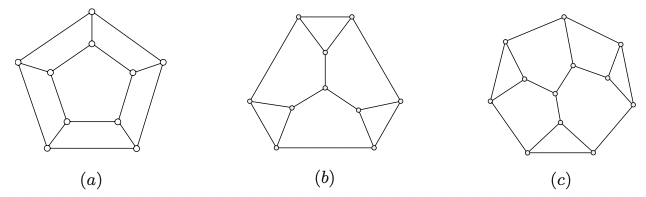
\includegraphics[scale=0.70]{pics/graph1.png}
    \caption{a) Gráfica transitiva por vértices. b) Gráfica con tres órbitas. c) Gráfica con doce órbitas.}
    \label{fig:fig3}
\end{figure}
%---------------------------------

%---------------------------------
\begin{problem}{1.2.17}
Una gráfica simple es \textit{tránsitiva por aristas} si, para cualesquiera dos aristas $uv$ y $xy$, existe un automorfismo $\alpha$ tal que $\alpha(u) \alpha(v) = xy.$
\begin{itemize}
    \item[a)] Encuentre una gráfica que sea tránsitiva por vértices pero no transitiva por aristas. 
    \item[b)] Demuestre que cualquier gráfica sin vértices aislados y transitiva por aristas pero no transitiva por vértices es bipartita.
\end{itemize}
\end{problem}
\begin{proof}\text{ }
\begin{itemize}
    \item[a)] Consideremos la gráfica $G$ descrita en la Figura \ref{fig:fig1}. Es claro que, mediante rotaciones, esta gráfica es transitiva por vértices. Más aún, estas rotaciones muestran que existen a lo más dos órbitas de aristas: las aristas \textit{internas} y las aristas \textit{externas.} Afirmamos que esta gráfica tiene exactamente estas dos órbitas de aristas. Para ver esto, suponga por el contrario, que existe un automorfismo $\alpha$ de $G$ tal que $\alpha(v_1) \alpha(v_2) = v_1 v_3.$ Tenemos los siguientes dos casos: i) $\alpha(v_1) = v_1$ y $\alpha(v_2) = v_3$; ii) $\alpha(v_1) = v_3$ y $\alpha(v_2) = v_1$.
    
    Resolveremos únicamente el caso i) siendo el caso ii) similar. Sean $n(v_1) = \{v_2, v_3, v_6, v_7\}$, $n(v_2) = \{v_1, v_3, v_4, v_7\}$ y $n(v_3) = \{v_1, v_2, v_4, v_5\}$ los vértices adyacentes $v_1, v_2$ y $v_3$ respectivamente. Puesto que $\alpha(v_1) = v_1$ y $\alpha(v_2) = v_3$ y $\alpha$ preserva adyacencias, tenemos que
    
    $$\alpha(n(v_1)) = n(v_1)$$
    y
    $$\alpha(n(v_2)) = n(v_3).$$
    Por otro lado, $n(v_1) \cap n(v_2) = \{v_3, v_7\}$, por lo que $\alpha(\{v_3, v_7\}) \subset n(v_1) \cap n(v_3) =  \{v_2\}$. Pero esto es imposible, ya que $\alpha$ es inyectiva. Luego, la existencia del automorfismo $\alpha$ debe ser falsa. Concluimos que $G$ no es transitiva por aristas. 
    
    
\begin{figure}
    \centering
        
\tikzset{every picture/.style={line width=0.75pt}} %set default line width to 0.75pt        

\begin{tikzpicture}[x=0.75pt,y=0.75pt,yscale=-1,xscale=1]
%uncomment if require: \path (0,300); %set diagram left start at 0, and has height of 300

%Shape: Regular Polygon [id:dp9037339427358064] 
\draw   (402.7,145.65) -- (370.78,211.93) -- (299.05,228.31) -- (241.52,182.43) -- (241.52,108.86) -- (299.05,62.99) -- (370.78,79.36) -- cycle ;
%Straight Lines [id:da7988753876165546] 
\draw    (299.05,62.99) -- (402.7,145.65) ;
%Straight Lines [id:da569878667892397] 
\draw    (241.52,108.86) -- (370.78,79.36) ;
%Straight Lines [id:da781300776678792] 
\draw    (241.52,182.43) -- (370.78,211.93) ;
%Straight Lines [id:da9520351279044305] 
\draw    (241.52,108.86) -- (299.05,228.31) ;
%Straight Lines [id:da7577086501770416] 
\draw    (241.52,182.43) -- (299.05,62.99) ;
%Straight Lines [id:da9781128996508351] 
\draw    (299.05,228.31) -- (402.7,145.65) ;
%Straight Lines [id:da4179900613030797] 
\draw    (370.78,79.36) -- (370.78,211.93) ;
%Shape: Circle [id:dp2618920989311526] 
\draw  [fill={rgb, 255:red, 255; green, 255; blue, 255 }  ,fill opacity=1 ] (235.52,108.86) .. controls (235.52,105.54) and (238.21,102.86) .. (241.52,102.86) .. controls (244.84,102.86) and (247.52,105.54) .. (247.52,108.86) .. controls (247.52,112.17) and (244.84,114.86) .. (241.52,114.86) .. controls (238.21,114.86) and (235.52,112.17) .. (235.52,108.86) -- cycle ;
%Shape: Circle [id:dp8793435086199656] 
\draw  [fill={rgb, 255:red, 255; green, 255; blue, 255 }  ,fill opacity=1 ] (293.05,62.99) .. controls (293.05,59.67) and (295.73,56.99) .. (299.05,56.99) .. controls (302.36,56.99) and (305.05,59.67) .. (305.05,62.99) .. controls (305.05,66.3) and (302.36,68.99) .. (299.05,68.99) .. controls (295.73,68.99) and (293.05,66.3) .. (293.05,62.99) -- cycle ;
%Shape: Circle [id:dp21677476420586805] 
\draw  [fill={rgb, 255:red, 255; green, 255; blue, 255 }  ,fill opacity=1 ] (235.52,182.43) .. controls (235.52,179.12) and (238.21,176.43) .. (241.52,176.43) .. controls (244.84,176.43) and (247.52,179.12) .. (247.52,182.43) .. controls (247.52,185.75) and (244.84,188.43) .. (241.52,188.43) .. controls (238.21,188.43) and (235.52,185.75) .. (235.52,182.43) -- cycle ;
%Shape: Circle [id:dp6578914967481373] 
\draw  [fill={rgb, 255:red, 255; green, 255; blue, 255 }  ,fill opacity=1 ] (293.05,228.31) .. controls (293.05,224.99) and (295.73,222.31) .. (299.05,222.31) .. controls (302.36,222.31) and (305.05,224.99) .. (305.05,228.31) .. controls (305.05,231.62) and (302.36,234.31) .. (299.05,234.31) .. controls (295.73,234.31) and (293.05,231.62) .. (293.05,228.31) -- cycle ;
%Shape: Circle [id:dp08096057364494613] 
\draw  [fill={rgb, 255:red, 255; green, 255; blue, 255 }  ,fill opacity=1 ] (364.78,211.93) .. controls (364.78,208.62) and (367.46,205.93) .. (370.78,205.93) .. controls (374.09,205.93) and (376.78,208.62) .. (376.78,211.93) .. controls (376.78,215.25) and (374.09,217.93) .. (370.78,217.93) .. controls (367.46,217.93) and (364.78,215.25) .. (364.78,211.93) -- cycle ;
%Shape: Circle [id:dp751915779747381] 
\draw  [fill={rgb, 255:red, 255; green, 255; blue, 255 }  ,fill opacity=1 ] (364.78,79.36) .. controls (364.78,76.04) and (367.46,73.36) .. (370.78,73.36) .. controls (374.09,73.36) and (376.78,76.04) .. (376.78,79.36) .. controls (376.78,82.67) and (374.09,85.36) .. (370.78,85.36) .. controls (367.46,85.36) and (364.78,82.67) .. (364.78,79.36) -- cycle ;
%Shape: Circle [id:dp13565241066130518] 
\draw  [fill={rgb, 255:red, 255; green, 255; blue, 255 }  ,fill opacity=1 ] (396.7,145.65) .. controls (396.7,142.33) and (399.39,139.65) .. (402.7,139.65) .. controls (406.01,139.65) and (408.7,142.33) .. (408.7,145.65) .. controls (408.7,148.96) and (406.01,151.65) .. (402.7,151.65) .. controls (399.39,151.65) and (396.7,148.96) .. (396.7,145.65) -- cycle ;

% Text Node
\draw (293,42.4) node [anchor=north west][inner sep=0.75pt]  [font=\small]  {$v_{1}$};
% Text Node
\draw (369,60.4) node [anchor=north west][inner sep=0.75pt]  [font=\small]  {$v_{2}$};
% Text Node
\draw (412,137.4) node [anchor=north west][inner sep=0.75pt]  [font=\small]  {$v_{3}$};
% Text Node
\draw (378.78,215.33) node [anchor=north west][inner sep=0.75pt]  [font=\small]  {$v_{4}$};
% Text Node
\draw (290.05,234.71) node [anchor=north west][inner sep=0.75pt]  [font=\small]  {$v_{5}$};
% Text Node
\draw (217.52,176.83) node [anchor=north west][inner sep=0.75pt]  [font=\small]  {$v_{6}$};
% Text Node
\draw (219,99.4) node [anchor=north west][inner sep=0.75pt]  [font=\small]  {$v_{7}$};
\end{tikzpicture}

    \caption{Gráfica transitiva por vértices pero no por aristas.}
    \label{fig:fig1}
    \end{figure}
    
    \item[b)] Sea $x$ un vértice de $G$. Como $G$ no tiene vértices aislados, existe un vértice $y$ de $G$ tal que $xy \in E(G).$ Sean $X$ y $Y$ las órbitas de $x$ y $y$ respectivamente. Dado que $G$ es transitiva por aristas y no tiene vértices aislados, tenemos que $X \cup Y = V(G).$ Más aún, $X \cap Y = \varnothing$, pues de lo contrario $G$ sería transitiva por vértices. 
    
    %Demostraremos que $X \cup Y = V(G)$. Si $u \in V(G),$ como este no es un vértice aislado, existe $v\in V(G)$ tal que $uv\in E(G).$ Por transitividad de aristas, existe un automorfismo $\alpha$ de $G$ tal que $\alpha(u)\alpha(v) = xy$. Luego, $u  \in X$ o $u \in Y$, obteniendo lo deseado. Por otro lado, $X \cap Y = \emptyset$, pues $G$ no es transitiva por vértices. Por tanto, $X$ y $Y$ es una partición del conjunto de vértices de $G.$
    
    Para ver que $G$ es bipartita, sea $u v \in E(G).$ Por transitividad de aristas, existe un automorfismo $\alpha$ de $G$ tal que $\alpha(x) \alpha(y) = u v.$ Pero entonces $u\in X$ y $v \in Y$ o $u \in Y$ y $v \in X$. Esto muestra que toda arista de $G$ tiene un extremo en $X$ y otro en $Y$. Por tanto $G$ es bipartita. 
\end{itemize}
\end{proof}

%---------------------------------

%---------------------------------
\begin{problem}{1.3.8}
Sea $m$ y $n$ enteros positivos, donde $n > 2m$. La \textit{gráfica Kneser} $KG_{m,n}$ es la gráfica cuyos vértices son los $m-$subconjuntos de un $n-$conjunto $S$, en la cual, dos subconjuntos son adyacentes si y solo si su intersección es vacía. Demuestre que:
\begin{itemize}
    \item[a)] $KG_{1,n} \simeq K_n$, $n \geq 3$;
    \item[b)] $KG_{2,n}$ es isomorfa al complemento de $L(K_n)$, $n \geq 5.$
\end{itemize}
\end{problem}
\begin{proof}\text{ }
\begin{itemize}
    \item[a)] Sean $\{i\}$, $\{j\}$, $1\leq i < j \leq n$, dos vértices distintos de $KG_{1,n}$. Como $\{i\} \cap \{j\} = \emptyset$, entonces estos vértices son adyacentes. De manera que cualquier par de vértices en $KG_{1,n}$ son adyacentes. Como $v(KG_{1,n}) = n$, lo anterior implica que $KG_{1,n}$ es isomorfa a la gráfica completa $K_n$.
    
    \item[b)] Por simplicidad escribamos  $G = \overline{L(K_n)}$. Note que $V(G) = \{u_i u_j: u_i u_j \in E(K_n) \}$ y $E(G) = \{[u_i u_j][u_r u_s]: u_i u_j \text{ y } u_r u_s \text{ no tienen un vértice en común} \}.$ \footnote{Observe que $u_i u_j$ es el mismo vértice que $u_j, u_i.$ en $G.$} Definamos el mapeo $\theta: V(KG_{2,n}) \rightarrow V(G)$ como 

    $$\theta(\{i,j\}) = u_iu_j.$$
    
    Es claro que mapeo es una biyección. Sea $\{i,j\}\{r,s\}$ una arista de $KG_{2,n}$. Como $\theta(\{i,j\}) = u_i u_j$,  $\theta(\{r,s\}) = u_r u_s$ y $\{i,j\} \cap \{r,s\} = \emptyset$, entonces $u_i u_j$ y $u_r u_s$ no tienen vértices en común en $K_n.$ Esto implica que $u_i u_j$ y $u_r u_s$ son adyacentes en $G.$ Por tanto, el mapeo $\theta$ es un isomorfismo.


%Observe que, si $V(K_n) = \{u_1, \ldots, u_n\}$, entonces $V(G) = \{ v_{ij} : u_i \text{ no es adyacente a } u_j \text{ en } K_n \}$. Consideremos el mapeo $\theta: V(KG_{2,n}) \rightarrow V(G)$ definido como 
    %$$\theta(\{i,j\}) = v_{ij}.$$
    %Afirmamos que $\theta$ preserva adyacencias. Sea $\{i,j\} \{r, s\}$ una arista en $V(KG_{2,n})$. Por definición, $\{i, j\} \cap \{r,s\} = \emptyset.$ Luego, $u_i, u_j, u_r$ y $u_s$  son todos vértices distintos. Por tanto, no 
    
\end{itemize}

\end{proof}

%---------------------------------

%\section*{Apéndice}

%\begin{prop}\label{'prop1'}
%Si $G$ es simple y no conexa y $\{X,Y\}$ es una partición de $V(G)$, entonces existen $x\in X$ y $y\in Y$ no adyacentes. 
%\end{prop}
%\begin{proof}
%Como $G$ es no conexa, existe una partición $\{X^\prime, Y^\prime\}$ de $V(G)$ tal que ningún vértice de $X^\prime$ es adyacente a ningún vértice de $Y^\prime$. Sea $\{X, Y\}$ una partición cualquiera de $V(G)$ con $X$ y $Y$ distintos del vacío. Si $\{X, Y\} = \{X^\prime, Y^\prime \}$, el resultado se sigue inmediatamente. Suponga que las particiones anteriores son distintas. Vea que $X = (X \cap X^\prime) \cup (X \cap Y^\prime)$, por lo que sin pérdida de generalidad podemos asumir que $X \cap X^\prime \neq \emptyset.$ Afirmamos que $Y \cap Y^\prime \neq \emptyset.$ De lo contrario, como $Y = V(G)-X$, tenemos que $X \cup Y \subset $ 
%\end{proof}

\printbibliography


\end{document}